\section{Complete extended sampling results}\label{app:extension-results}
Figure~\ref{fig:extension-sampling} includes every oracle sampling configuration at $P=8192,U=20$. Across the full 1,080-cell oracle extension, all 600 full-factor or tail-controlled cells have finite normalizers; all 480 raw unbiased cells have infinite normalizers. In particular, $M\in\{2,4,8\}$ remains below the finite thresholds at $G=64$ for these tails. The statement is a certificate calculation, not an inference from observed particle errors.

\begin{figure}[p]
 \centering
 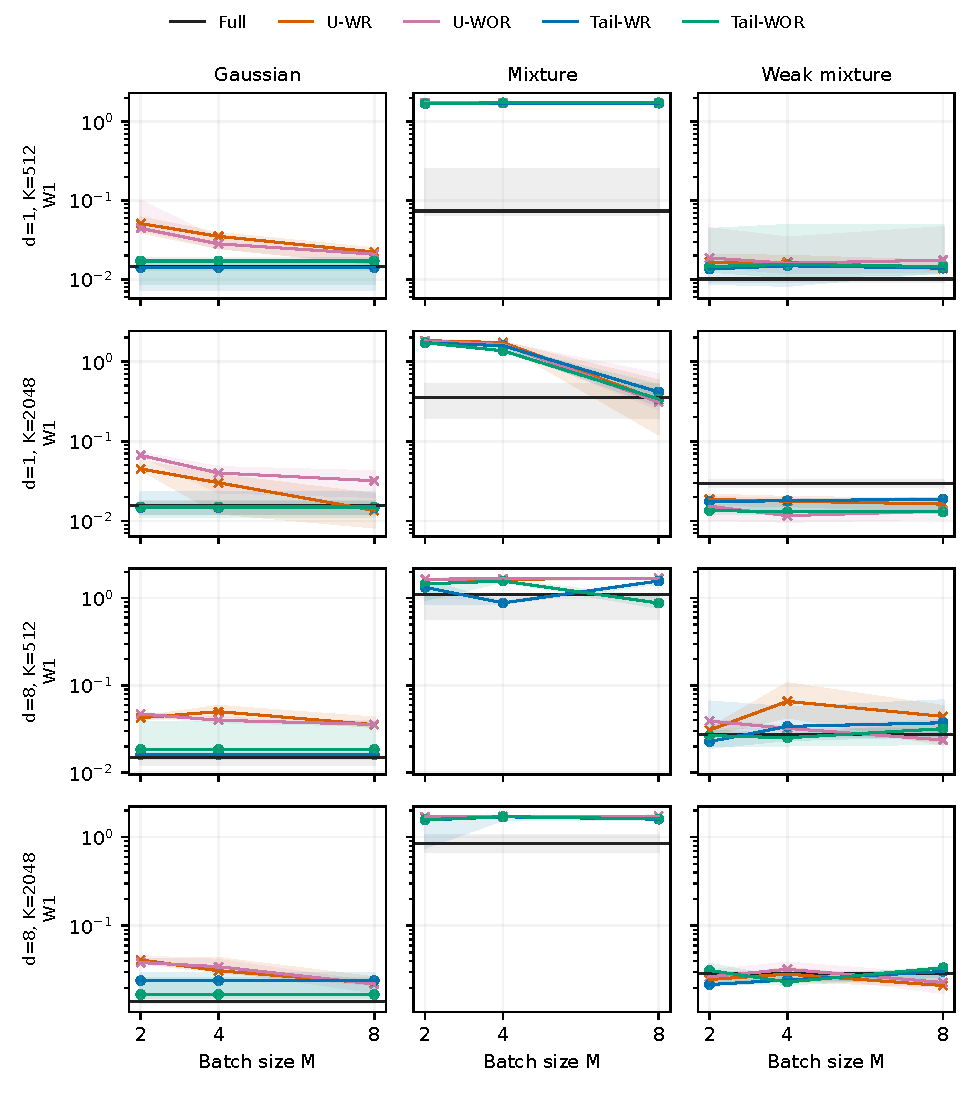
\includegraphics[width=\linewidth]{figures/extension_sampling.pdf}
 \caption{Complete oracle batch-size comparison. Curves show median marginal W1 and interquartile ranges across five seeds. The horizontal black line and band show the full-factor median and interquartile range. Circles denote finite normalizers and crosses infinite ones. Every row uses $G=64,P=8192,U=20$; its dimension and grid size are labeled at left. All four subsampled methods and all three batch sizes are shown.}
 \label{fig:extension-sampling}
\end{figure}

\subsection{Particle count and terminal-noise sensitivity}
Figure~\ref{fig:extension-sensitivity} reports the full sweep at $G=64,d=8,K=512,M=4$. Increasing particles does not guarantee monotone improvement over this range. For the ordinary mixture, full-factor mean W1 decreases from $0.881$ at $P=8192$ to $0.650$ at $P=131072$, while tail control without replacement remains poor, with mean W1 $1.440$ and $1.470$ respectively. For the weak mixture, raw with-replacement weighting improves from $0.0704$ to $0.0098$ while remaining nonintegrable, whereas finite tail control without replacement has mean W1 $0.0250$, $0.0194$ and $0.0357$ across the three particle counts. Thus increasing particles does not repair a failed population certificate, and the observed finite methods need not improve monotonically.

Changing $U$ from 10 through 20 to 30 at fixed $K$ leaves the full-factor and tail-control certificates finite and the raw certificates infinite in every tested cell. Full-factor mean W1 is $0.0265$, $0.0280$ and $0.0282$ for the weak mixture, and $0.801$, $0.881$ and $0.711$ for the ordinary mixture. Because this intervention changes the entire time grid as well as the initialization level, these data cannot identify an initialization-only effect.

\begin{figure}[p]
 \centering
 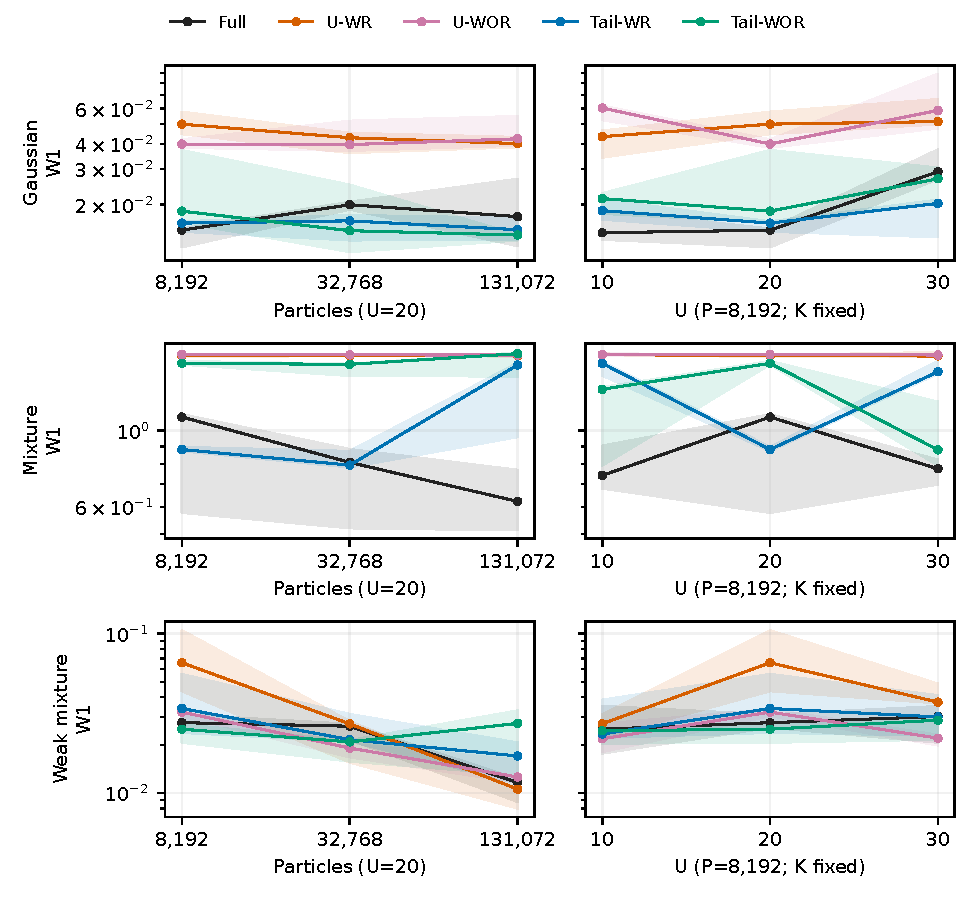
\includegraphics[width=\linewidth]{figures/extension_sensitivity.pdf}
 \caption{Complete particle-count and terminal-noise sweeps, with median marginal W1 and interquartile ranges across five seeds. Here circles mark every measured setting and do not encode validity: Full, Tail-WR and Tail-WOR are finite throughout; U-WR and U-WOR are infinite throughout. Left panels vary $P$ at $U=20$; right panels vary $U$ at $P=8192$. Both hold $K=512$ fixed.}
 \label{fig:extension-sensitivity}
\end{figure}

\subsection{Coarser learned-posterior grid}
Figure~\ref{fig:learned-coarse} retains all 25 pairs at $K=512$. Both grids have the same certificate classifications, while endpoint errors depend on the grid. Tables~\ref{tab:learned-512} and~\ref{tab:learned-2048} report all configuration means and standard deviations; the released CSVs contain every individual cell, KS and moment diagnostics, prediction time and sampler time. The 100 distinct learned compositions are also retained individually.

\begin{figure}[htbp]
 \centering
 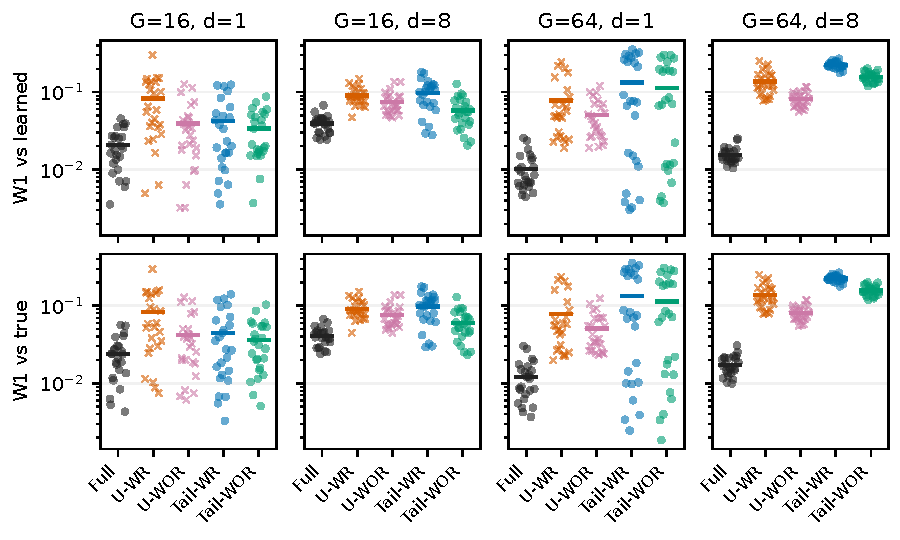
\includegraphics[width=\linewidth]{figures/learned_results_coarse.pdf}
 \caption{Complete learned-posterior comparison at $K=512$, using the same display and validity conventions as Figure~\ref{fig:learned}. All training and dataset seeds are included.}
 \label{fig:learned-coarse}
\end{figure}
\begin{table}[htbp]
 \centering
 \caption{Complete learned-posterior results at $K=512$. W1 values are means $\pm$ sample standard deviations across 25 crossed checkpoint/dataset pairs. Time is mean recorded sampler seconds. F and I denote finite and infinite population normalizers.}
 \label{tab:learned-512}
 \small
 \begin{tabular}{rrlcllr}
 \toprule
 $G$ & $d$ & Method & Domain & W1 vs learned & W1 vs true & Seconds\\
 \midrule

16 & 1 & Full & F & $0.0207\pm0.0116$ & $0.0240\pm0.0144$ & 0.59\\
16 & 1 & U-WR & I & $0.0828\pm0.0679$ & $0.0824\pm0.0690$ & 0.76\\
16 & 1 & U-WOR & I & $0.0392\pm0.0336$ & $0.0417\pm0.0350$ & 0.73\\
16 & 1 & Tail-WR & F & $0.0420\pm0.0391$ & $0.0450\pm0.0415$ & 0.99\\
16 & 1 & Tail-WOR & F & $0.0339\pm0.0223$ & $0.0364\pm0.0253$ & 1.00\\
\midrule
16 & 8 & Full & F & $0.0392\pm0.0103$ & $0.0408\pm0.0111$ & 1.94\\
16 & 8 & U-WR & I & $0.0907\pm0.0238$ & $0.0915\pm0.0253$ & 1.14\\
16 & 8 & U-WOR & I & $0.0740\pm0.0253$ & $0.0755\pm0.0257$ & 1.23\\
16 & 8 & Tail-WR & F & $0.0969\pm0.0420$ & $0.0978\pm0.0416$ & 1.26\\
16 & 8 & Tail-WOR & F & $0.0578\pm0.0258$ & $0.0598\pm0.0258$ & 1.36\\
\midrule
64 & 1 & Full & F & $0.0102\pm0.0057$ & $0.0121\pm0.0070$ & 1.16\\
64 & 1 & U-WR & I & $0.0776\pm0.0673$ & $0.0779\pm0.0671$ & 0.79\\
64 & 1 & U-WOR & I & $0.0503\pm0.0289$ & $0.0508\pm0.0285$ & 0.80\\
64 & 1 & Tail-WR & F & $0.1336\pm0.1299$ & $0.1343\pm0.1301$ & 0.99\\
64 & 1 & Tail-WOR & F & $0.1130\pm0.1096$ & $0.1138\pm0.1096$ & 0.98\\
\midrule
64 & 8 & Full & F & $0.0155\pm0.0037$ & $0.0173\pm0.0051$ & 6.56\\
64 & 8 & U-WR & I & $0.1365\pm0.0488$ & $0.1368\pm0.0488$ & 1.19\\
64 & 8 & U-WOR & I & $0.0807\pm0.0180$ & $0.0808\pm0.0182$ & 1.33\\
64 & 8 & Tail-WR & F & $0.2246\pm0.0219$ & $0.2248\pm0.0206$ & 1.33\\
64 & 8 & Tail-WOR & F & $0.1569\pm0.0225$ & $0.1573\pm0.0226$ & 1.48\\
\bottomrule
\end{tabular}
\end{table}

\begin{table}[htbp]
 \centering
 \caption{Complete learned-posterior results at $K=2048$. W1 values are means $\pm$ sample standard deviations across 25 crossed checkpoint/dataset pairs. Time is mean recorded sampler seconds. F and I denote finite and infinite population normalizers.}
 \label{tab:learned-2048}
 \small
 \begin{tabular}{rrlcllr}
 \toprule
 $G$ & $d$ & Method & Domain & W1 vs learned & W1 vs true & Seconds\\
 \midrule

16 & 1 & Full & F & $0.0192\pm0.0108$ & $0.0222\pm0.0131$ & 2.27\\
16 & 1 & U-WR & I & $0.0251\pm0.0177$ & $0.0275\pm0.0175$ & 2.80\\
16 & 1 & U-WOR & I & $0.0208\pm0.0129$ & $0.0248\pm0.0143$ & 2.72\\
16 & 1 & Tail-WR & F & $0.0256\pm0.0306$ & $0.0298\pm0.0320$ & 4.05\\
16 & 1 & Tail-WOR & F & $0.0208\pm0.0136$ & $0.0241\pm0.0156$ & 3.86\\
\midrule
16 & 8 & Full & F & $0.0402\pm0.0140$ & $0.0424\pm0.0157$ & 7.70\\
16 & 8 & U-WR & I & $0.0572\pm0.0253$ & $0.0579\pm0.0251$ & 4.35\\
16 & 8 & U-WOR & I & $0.0400\pm0.0130$ & $0.0419\pm0.0148$ & 4.74\\
16 & 8 & Tail-WR & F & $0.0504\pm0.0208$ & $0.0517\pm0.0213$ & 4.94\\
16 & 8 & Tail-WOR & F & $0.0474\pm0.0231$ & $0.0486\pm0.0242$ & 5.38\\
\midrule
64 & 1 & Full & F & $0.0125\pm0.0080$ & $0.0135\pm0.0092$ & 4.51\\
64 & 1 & U-WR & I & $0.0335\pm0.0259$ & $0.0344\pm0.0278$ & 3.07\\
64 & 1 & U-WOR & I & $0.0269\pm0.0197$ & $0.0291\pm0.0193$ & 2.91\\
64 & 1 & Tail-WR & F & $0.0610\pm0.0586$ & $0.0616\pm0.0590$ & 3.92\\
64 & 1 & Tail-WOR & F & $0.0487\pm0.0402$ & $0.0497\pm0.0409$ & 3.94\\
\midrule
64 & 8 & Full & F & $0.0189\pm0.0073$ & $0.0201\pm0.0073$ & 26.09\\
64 & 8 & U-WR & I & $0.1006\pm0.0337$ & $0.1012\pm0.0335$ & 4.56\\
64 & 8 & U-WOR & I & $0.0448\pm0.0130$ & $0.0462\pm0.0130$ & 5.14\\
64 & 8 & Tail-WR & F & $0.1276\pm0.0147$ & $0.1279\pm0.0151$ & 5.13\\
64 & 8 & Tail-WOR & F & $0.0907\pm0.0136$ & $0.0912\pm0.0129$ & 5.73\\
\bottomrule
\end{tabular}
\end{table}

